\documentclass[student]{ITRslides}

\addbibresource{ref.bib}
\graphicspath{{pics/}{logos/}}

\title{Control of a multi-robot cooperative team guided by a human operator}
\presenter{M. Angerer}

\supervisor{S. Musi\'c}
\typeofpres{Intermediate Presentation Master Thesis}



%%%%%%%%%%%%%%%%%%%%%%%%%%%%%%%%%%%%%%%%%%%%%%%%%%%%%%%%%%%%%%%%%%%%%%%%%%%%%%%%

\begin{document}


\begin{frame}
    \titlepage
\end{frame}

%\begin{frame}
%	\frametitle{Overview}
%    \tableofcontents%[hideallsubsections]%[pausesections]
%\end{frame}

\section{Introduction}

\begin{frame}
	\frametitle{Cooperative Manipulation Tasks}
		\begin{columns}
		\column{0.6\linewidth}
			\begin{figure}[htb]
			\centering
			%\psfrag{q1}[Bl][Bl]{\small $\alpha$}
			\includegraphics[width=0.98\textwidth]{mhi-meister45.jpg}
			\caption{Demonstration of MHI MEISTeR at 						Fukushima Daiichi 					Nuclear 						Power Station\cite{}}
			\end{figure} 
		\column{0.45\linewidth}
			\begin{itemize}
				\item transportation of large/heavy objects
	\item assembly of multiple parts 
	\item grasping an object without rigid fixture 
	\item deforming a flexible object
	\item coordinated use of tools
			\end{itemize}
			\end{columns}
\end{frame}

\begin{frame}
	\frametitle{Problem Formulation}

	\begin{itemize}
		\item Precise and stable control especially during free-motion/contact transition
		\item Perform friction based grasps
		\item Ability to operate in remote/hazardous areas
		\item Intuitive high-level control for the human operator
	\end{itemize}

\end{frame}

\begin{frame}
	\frametitle{Related Work: Cooperative Manipulation}
	\begin{itemize}
		\item Hybrid Position/Force Control \varcite{Wen_92}{1} \cite{Hsu_93}
		\begin{itemize}
			\item Control of motion and internal forces
			\item Viable for stable contacts
		\end{itemize}
		\item Impedance Control
		\begin{itemize}
			\item Object-Environment \cite{Schneider_92}
			\item Internal Force-based\cite{Bonitz_96}
			\item Combined \cite{Caccavale_01,Caccavale_08}
			\item Internal + Object force feed-forward \cite{DePascali_15}
		\end{itemize}
		\item Formation Control \cite{Sieber_15}
	\end{itemize}
\end{frame}

\section{Approach}

\begin{frame}
	\frametitle{Intrinsically Passive Control (IPC)}
	\begin{columns}
		\column{0.4\linewidth}
			
	
		\begin{itemize}
			\item High-level Supervisor and low-level IPC
			\item IPC + robot: passive
			\item Power provided by Supervisor
			\item Environment assumed passive
		\end{itemize}

		
		\column{0.58\linewidth}
             \begin{figure}[htb]
			\centering
			%\psfrag{q1}[Bl][Bl]{\small $\alpha$}
			\includegraphics[width=0.9\textwidth]{IPCoverview.png}
			\caption{Overview of the IPC architecture 								\cite{Stramigioli_01}}
			\end{figure}
		
			
		\end{columns}
\end{frame}

\begin{frame}
	\frametitle{Structure of the IPC}
\begin{columns}
		\column{0.5\linewidth}
			
	
		\begin{itemize}
			\item Spring-mass-damper system
			\item Simulated virtual object
			\item Manipulators modelled by inertias
			\item Potential (inertia) and kinetic (springs) energy
			\item Energy dissipation in damper: passivity
		\end{itemize}

		
		\column{0.5\linewidth}
             \begin{figure}[htb]
			\centering
			%\psfrag{q1}[Bl][Bl]{\small $\alpha$}
			\includegraphics[width=0.98\textwidth]{IPCsprings.png}
			\caption{Mass-spring-damper structure of the IPC 						\cite{Stramigioli_01}}
			\end{figure}
		
			
		\end{columns}
\end{frame}

\begin{frame}
	\frametitle{Grasping an object}
\begin{columns}
		\column{0.4\linewidth}
			
	
		\begin{itemize}
			\item Variable rest-length springs
			\item Rest-length: virtual object size
			\item Power provided by Supervisor
		\end{itemize}

		
		\column{0.62\linewidth}
             \begin{figure}[htb]
			\centering
			%\psfrag{q1}[Bl][Bl]{\small $\alpha$}
			\includegraphics[width=0.98\textwidth]{IPCobjects.png}
			\caption{Virtual and real object \cite{Wimboeck_08}}
			\end{figure}
		
			
		\end{columns}
\end{frame}

\begin{frame}
	\frametitle{The Supervisor}
	\begin{itemize}
			\item Two power ports per IPC-robot-system
			\item Human operator takes role of Supervisor
			\item Connected via delayed communication line
		\end{itemize}
\end{frame}

\begin{frame}
	\frametitle{Tele-operation}
	\begin{itemize}
			\item Preserving passivity
			\item Scattering or Wave variables
		\end{itemize}
\end{frame}

\section{Results}
\begin{frame}
	\frametitle{Grasping force optimization for friction contacts}
	\begin{columns}
	\column{0.6\textwidth}
	\begin{itemize}
	\item required contact normal force is dependent on tangential forces
	\item high tangential forces arise during acceleration
	\item other requirements: safety margin, maximum grasping force $\Rightarrow$ cost function
	\item linear matrix inequality (LMI) problem
	\end{itemize}
	\column{0.5\textwidth}

\begin{figure}[htb]
			\centering
			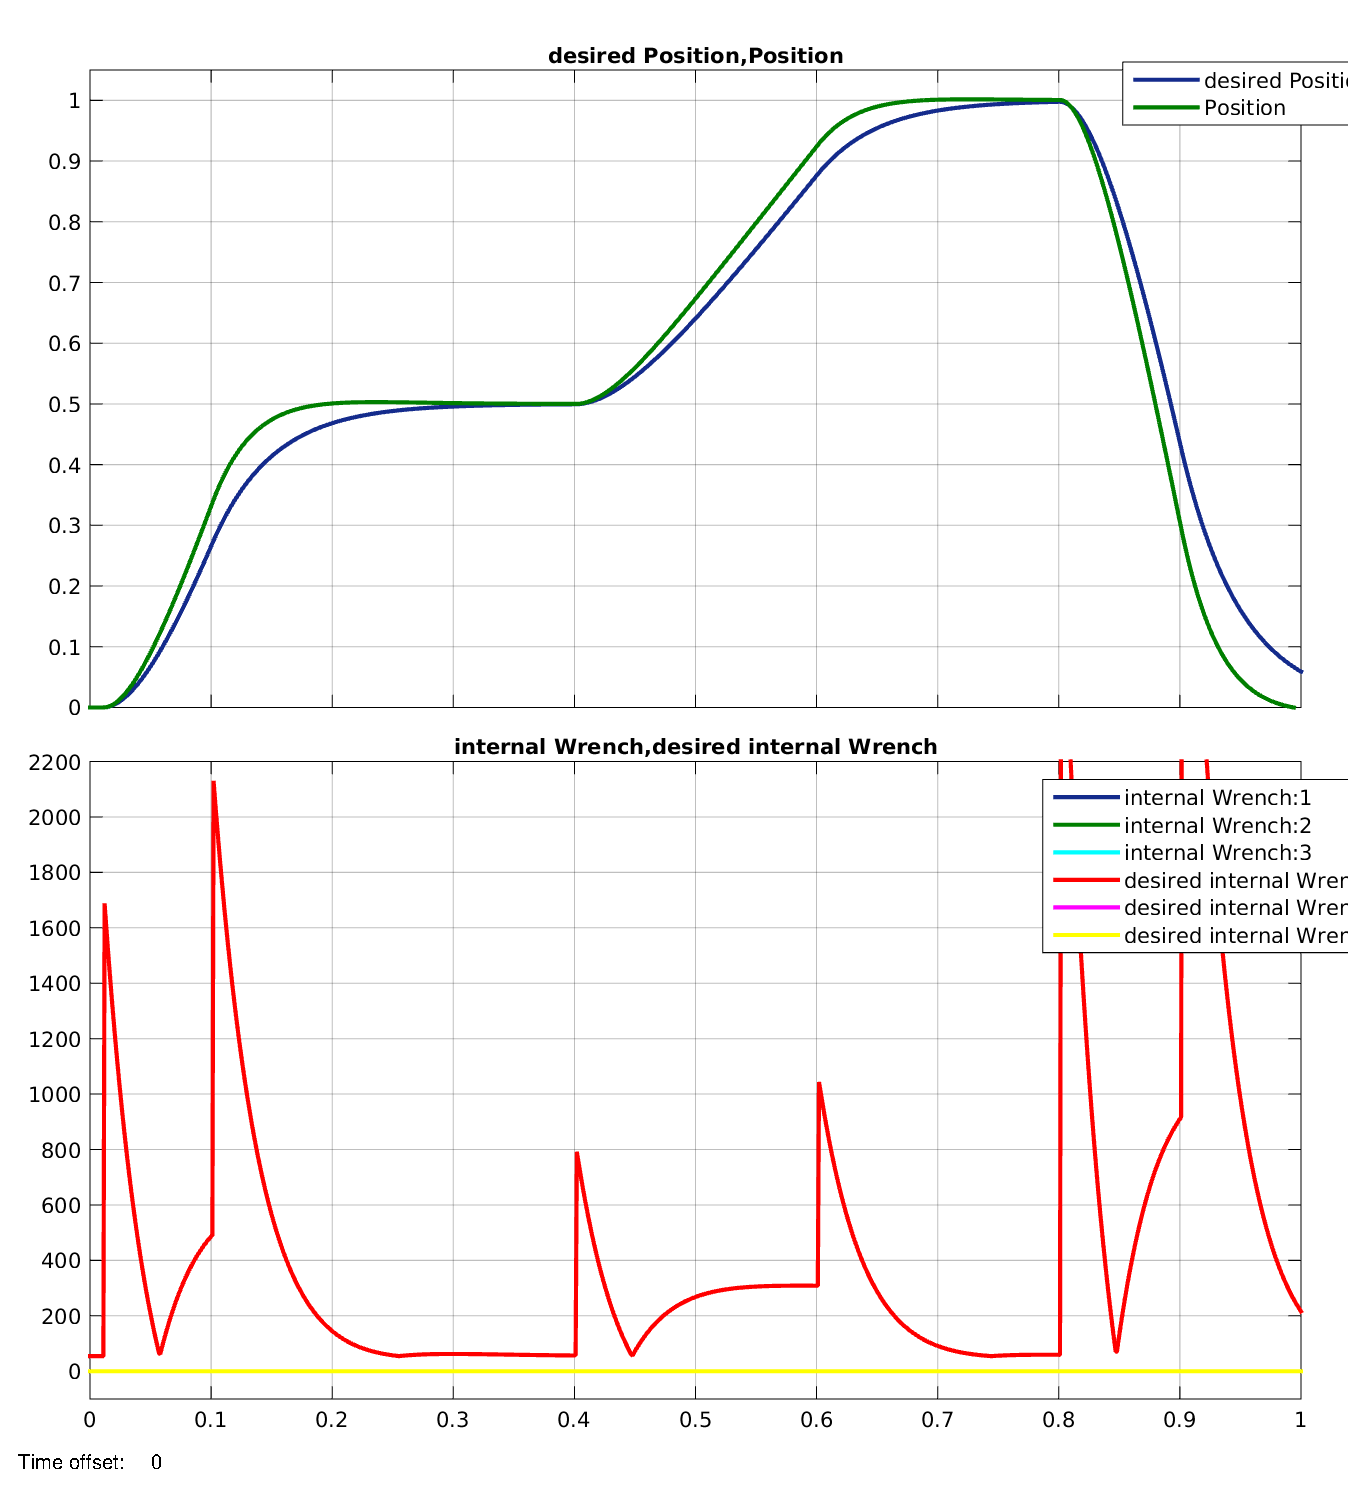
\includegraphics[width=0.9\textwidth]{Hanposforce.eps}
			\caption{Position, Internal wrench}
\end{figure}
\end{columns}
\end{frame}
\begin{frame}
	\frametitle{Comparison of Grasp Controllers 1}
Impedance-based reference trajectory generation \cite{Caccavale_01}
 \begin{figure}[htb]
			\centering
			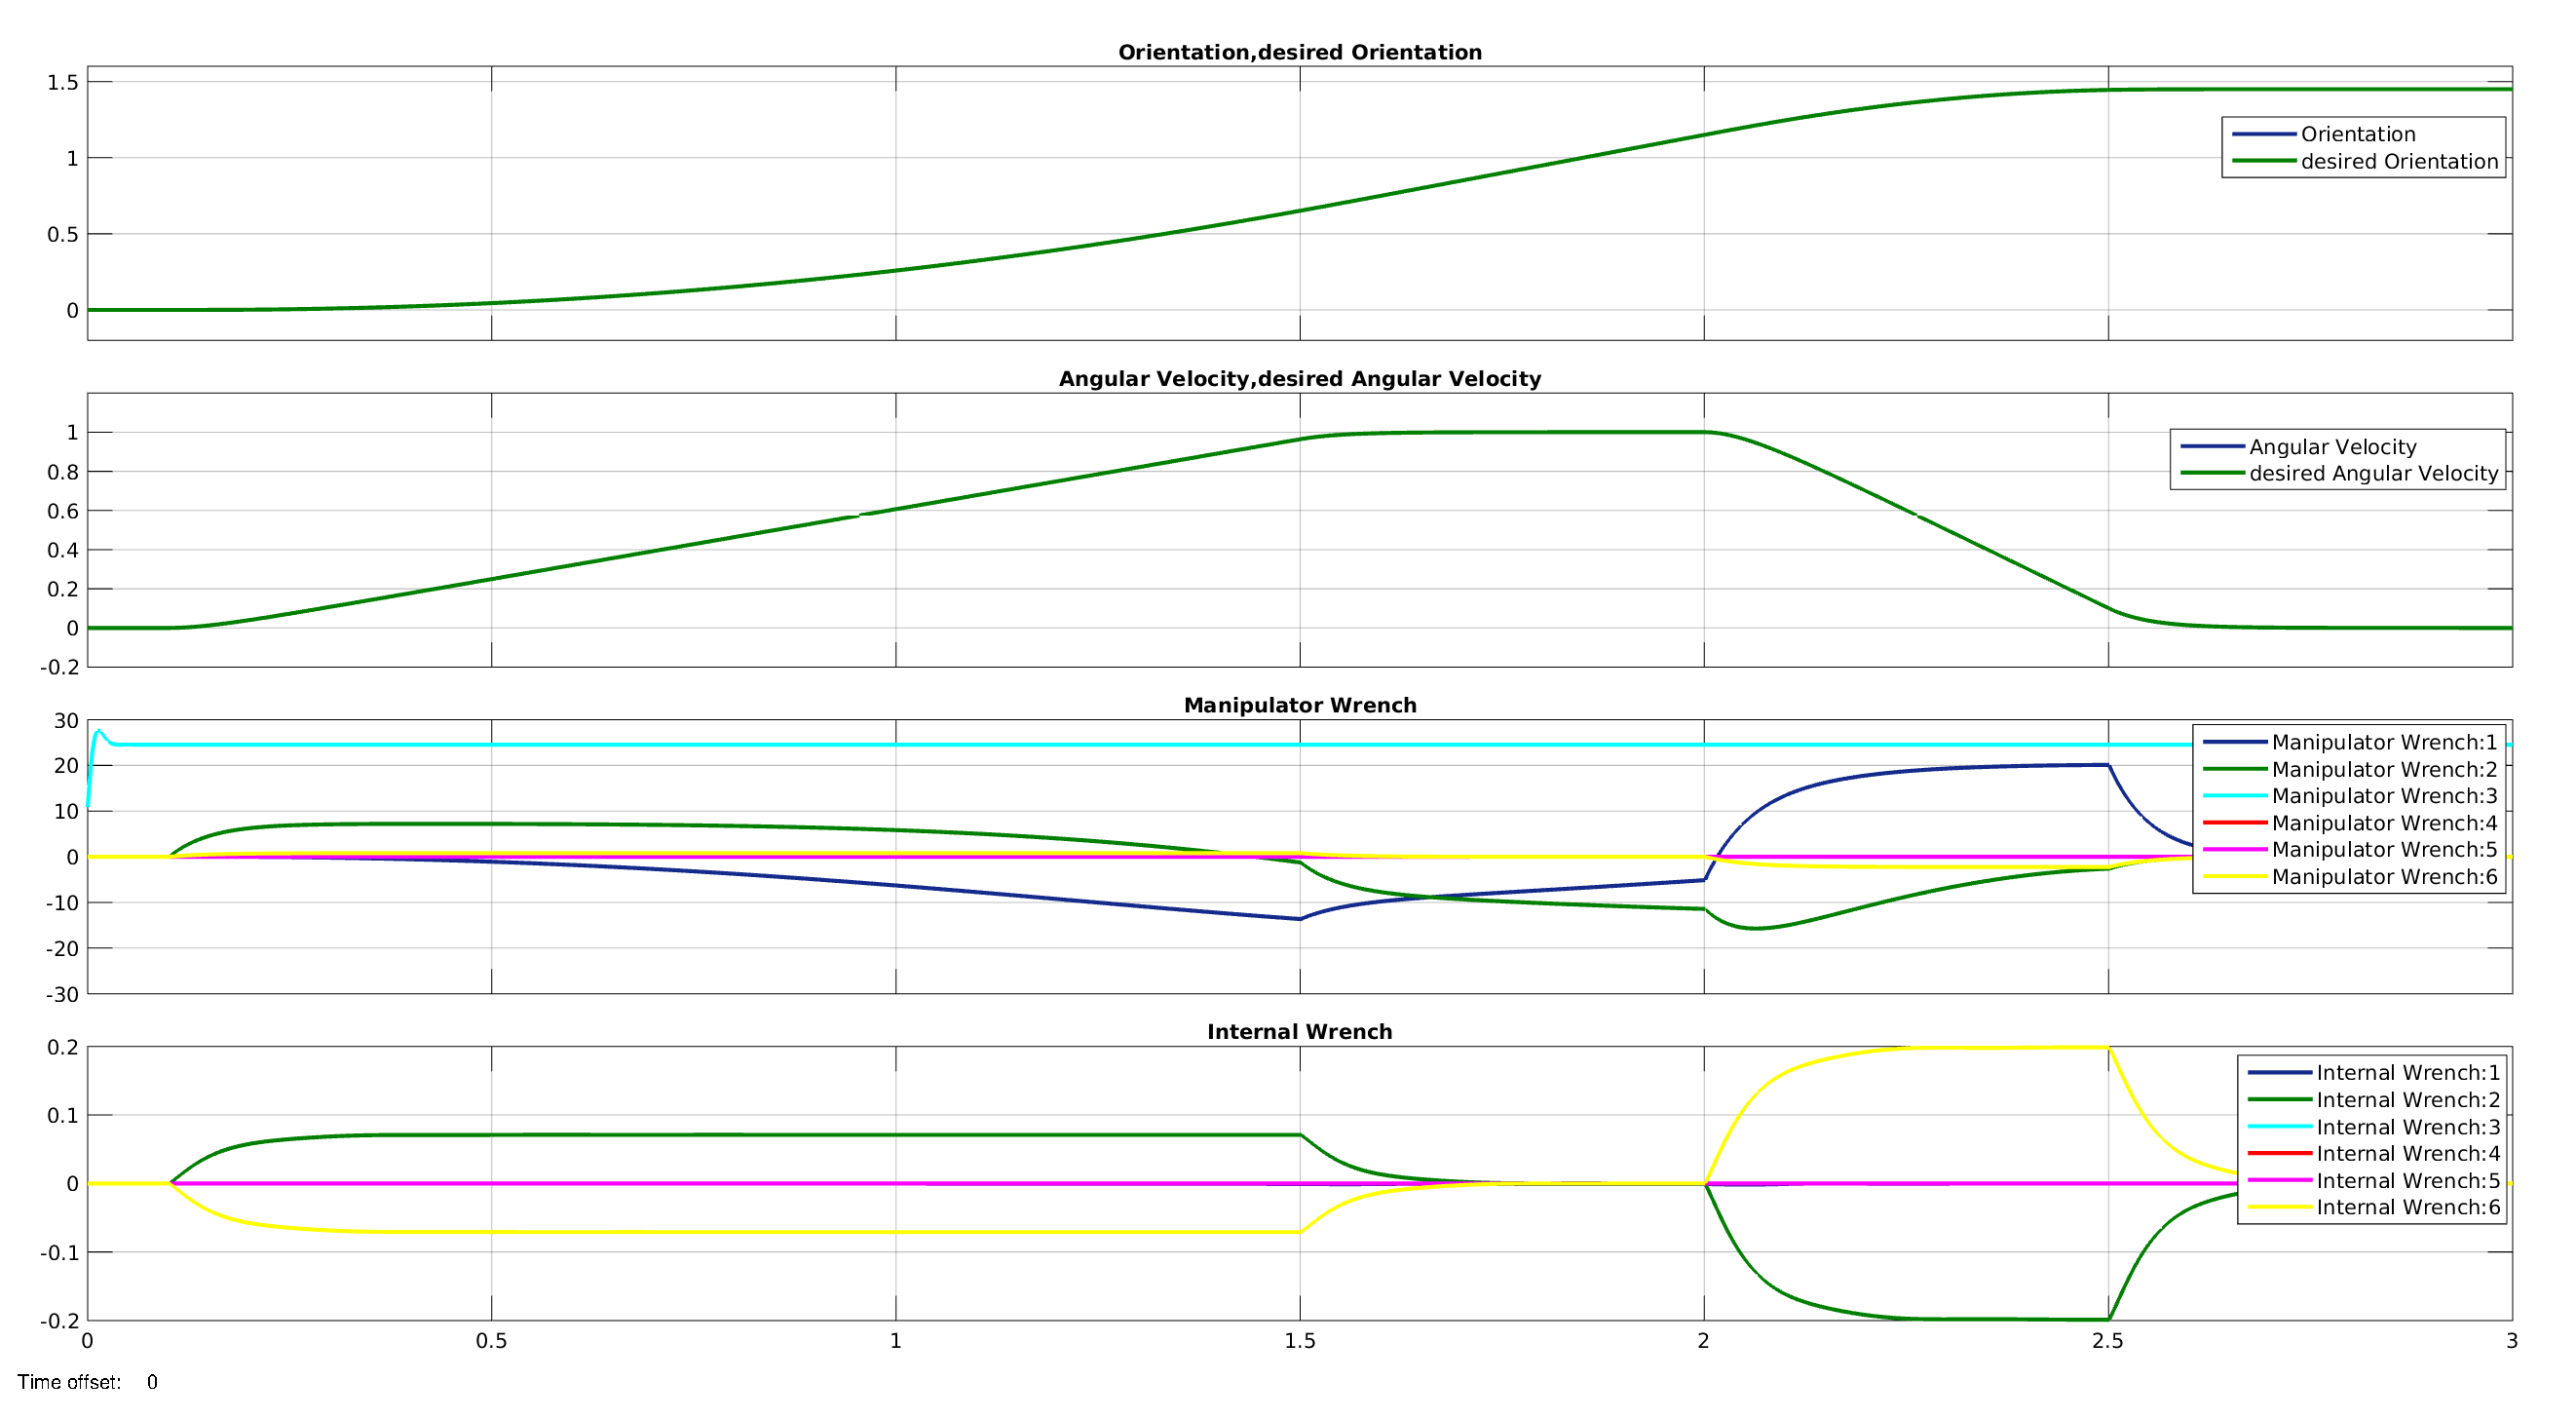
\includegraphics[width=0.9\textwidth]{Caccavaleorientation.eps}
			\caption{Position, Velocity, Manipulator wrench, Internal wrench}
\end{figure}
\end{frame}

\begin{frame}
	\frametitle{Comparison of Grasp Controllers 2}
Internal impedance control with object force-feedforward \cite{DePascali_15}
 \begin{figure}[htb]
			\centering
			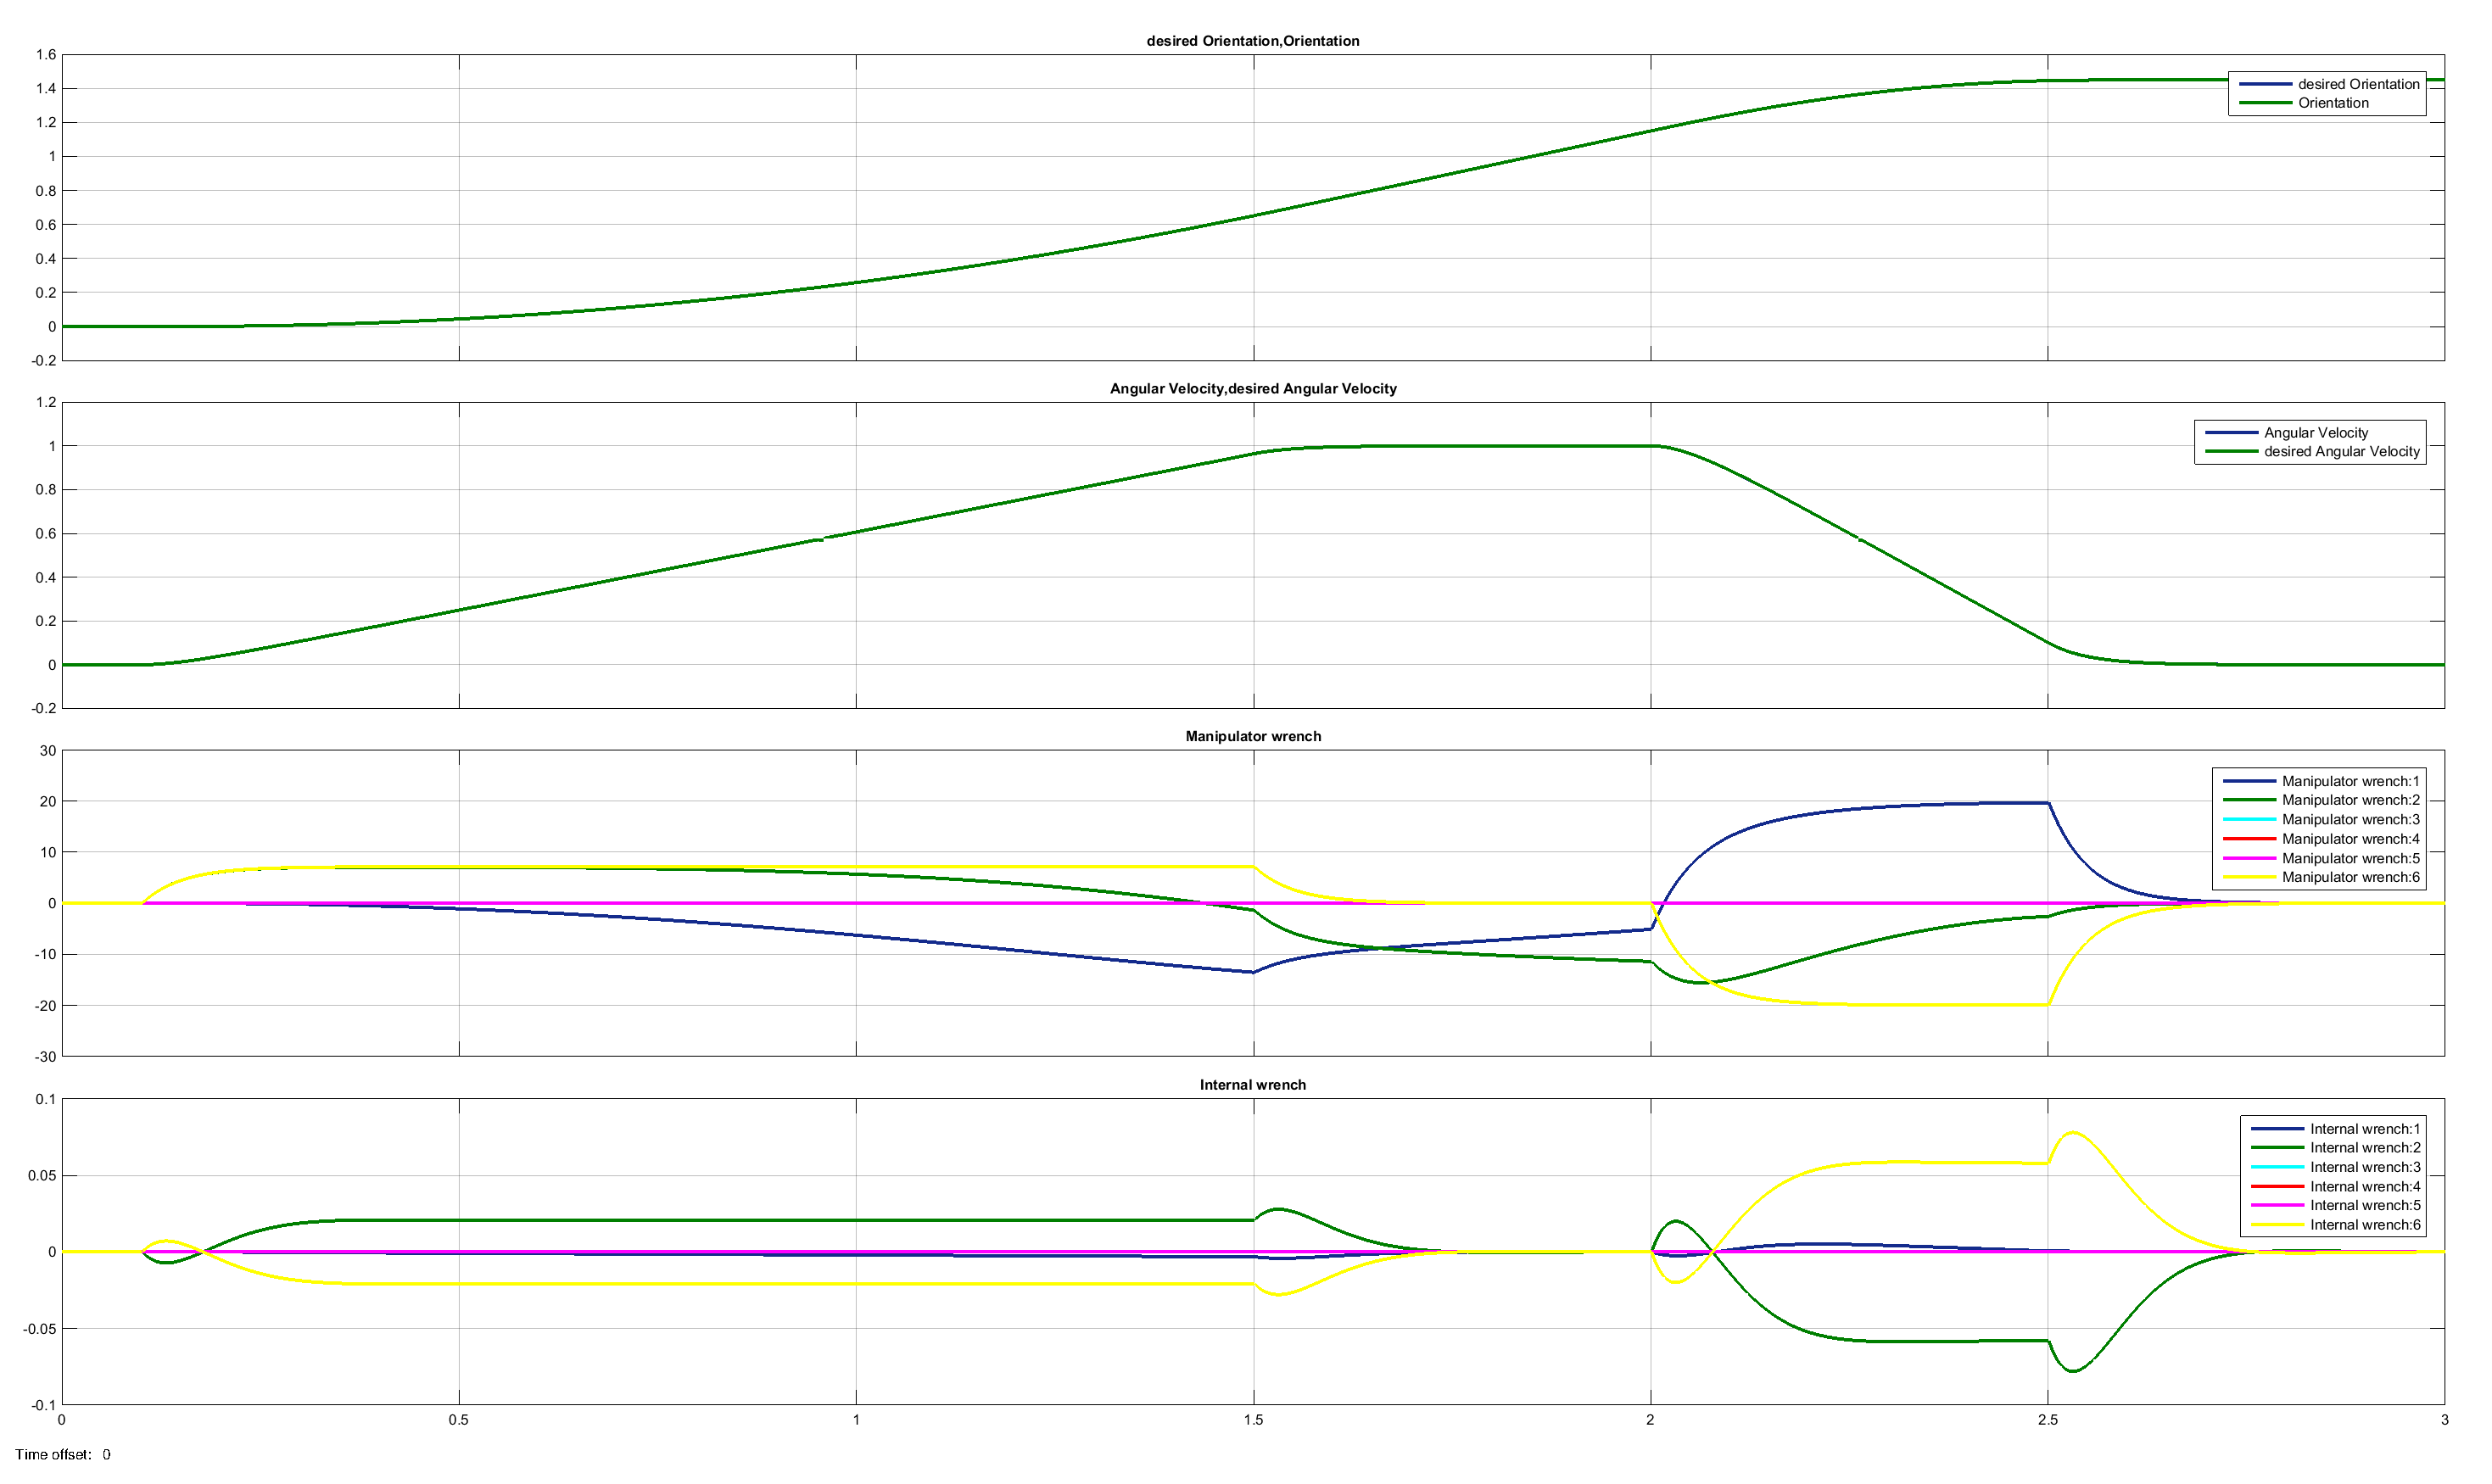
\includegraphics[width=0.9\textwidth]{Depascaliorientation.eps}
			\caption{Position, Velocity, Manipulator wrench, Internal wrench}
\end{figure}
\end{frame}

\section{Conclusion}

\begin{frame}
	\frametitle{Conclusion}
	...
\end{frame}
\appendix
%\nocite{buss11}
%\nocite{bauer09}
\begin{frame}
	\frametitle{References}
	%\tiny
	%\bibliographystyle{plain}
	%\bibliography{ref}
	\printbibliography
\end{frame}


\end{document}
